
\documentclass{article}
%%%%%%%%%%%%%%%%%%%%%%%%%%%%%%%%%%%%%%%%%%%%%%%%%%%%%%%%%%%%%%%%%%%%%%%%%%%%%%%%%%%%%%%%%%%%%%%%%%%%%%%%%%%%%%%%%%%%%%%%%%%%%%%%%%%%%%%%%%%%%%%%%%%%%%%%%%%%%%%%%%%%%%%%%%%%%%%%%%%%%%%%%%%%%%%%%%%%%%%%%%%%%%%%%%%%%%%%%%%%%%%%%%%%%%%%%%%%%%%%%%%%%%%%%%%%
\usepackage{geometry, tikz}



\newtheorem{theorem}{Theorem}
\newtheorem{acknowledgement}[theorem]{Acknowledgement}
\newtheorem{algorithm}[theorem]{Algorithm}
\newtheorem{axiom}[theorem]{Axiom}
\newtheorem{case}[theorem]{Case}
\newtheorem{claim}[theorem]{Claim}
\newtheorem{conclusion}[theorem]{Conclusion}
\newtheorem{condition}[theorem]{Condition}
\newtheorem{conjecture}[theorem]{Conjecture}
\newtheorem{corollary}[theorem]{Corollary}
\newtheorem{criterion}[theorem]{Criterion}
\newtheorem{definition}[theorem]{Definition}
\newtheorem{example}[theorem]{Example}
\newtheorem{exercise}[theorem]{Exercise}
\newtheorem{lemma}[theorem]{Lemma}
\newtheorem{notation}[theorem]{Notation}
\newtheorem{problem}[theorem]{Problem}
\newtheorem{proposition}[theorem]{Proposition}
\newtheorem{remark}[theorem]{Remark}
\newtheorem{solution}[theorem]{Solution}
\newtheorem{summary}[theorem]{Summary}
\newenvironment{proof}[1][Proof]{\noindent\textbf{#1.} }{\ \rule{0.5em}{0.5em}}

\geometry{left=1in,right=1in,top=1in,bottom=1in}

\newcommand{\ind}[1]{{\bf 1  }[ #1 ] }

\begin{document}

\begin{center}
\textbf{Econ 512}

\emph{Fall 2018}\\[1em]

Homework 4 -- Numerical Integration \\
Due 10/10/2018
\\[3em]
\end{center}

\bigskip

There are multiple ways to compute the mathematical constant $\pi$ via numerical integration. 
Probably the simplest is the ``dart-throwing'' method, which is a special case of an {\it accept-reject}
simulator. A somewhat more elegant approach comes from an integral representation. 
This homework will consider both.
Consider the quarter-circle arc of radius 1, centered at the origin inscribed within the unit square:



%\begin{figure}
\begin{center}
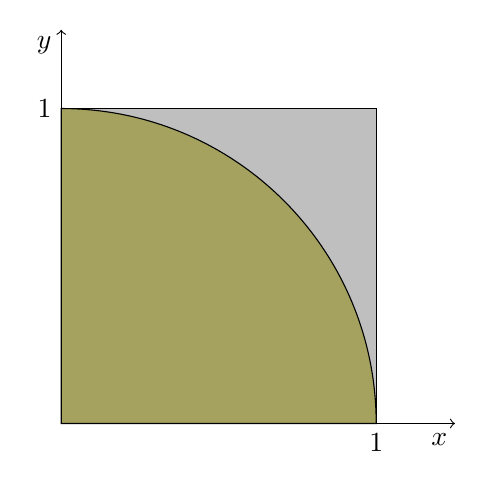
\begin{tikzpicture}[scale = 4]
\draw [<->] (0, 1.25) -- (0,0) -- (1.25, 0);
\draw [fill=lightgray] (0,1) rectangle (1, 0);
\filldraw[fill opacity=0.5,fill=olive] (0,0) -- (1, 0) arc (0:90:1) -- cycle;
\node [below] at (1,0) {$1$};
\node [below] at (1.2,0) {$x$};
\node [left] at (0, 1) {$1$};
\node[left] at (0, 1.2) {$y$};
\end{tikzpicture}
%\caption{Unit interval with arc}
\end{center}
%\end{figure}

Clearly, the area of the quarter-circle (green shaded area) is $\frac{\pi}{4}$ whereas the area of the unit square is 1.
For any point inside the unit square, we can tell whether it lies within the quarter-circle using the Pythagorean formula. 
That is, $(x,y)$ lies within the shaded are if $x^2 + y^2 \leq 1$. The dart-throwing method simply draws points uniformly from within the unit
square and accepts them when they lie within the circle and rejects them otherwise. The ratio of acceptances to total draws converges
to the area of the quarter circle. In other words, we can calculate $\pi$ using the double-integral,

$$ \pi = 4 \int_0^1 \int_0^1  \ind{ x^2 + y^2 \leq 1} dy dx. $$
 

\begin{enumerate} 

\item Write an algorithm that uses the dart-throwing method to approximate $\pi$ using a quasi-Monte Carlo approach to computing integrals. \\[1em]

The integral is approximately 3.1448 by using a quasi-Monte Carlo approach. \\[1em]

\item Write an algorithm that uses the dart-throwing method to approximate $\pi$ using a Newton-Cotes approach to computing integrals. \\[1em]

The integral is approximately 3.1417 by using a  Newton-Coates approach. \\[1em]

\end{enumerate}

However, all we are doing is calculating the area under the curve. From the same figure and again using Pythagorean formula, one can solve for $y$ as a function of $x$, $y = \sqrt{1 - x^2}$. Thus, we have a definition for $\pi$ based on a single dimensional integral, 

$$ \pi = 4 \int_0^1 \sqrt{1 - x^2} dx .$$

\begin{enumerate}
\setcounter{enumi}{2}
\item Approximate $\pi$ based on the above integral using a quasi-Monte Carlo approach. \\[1em]

$\pi$ is approximated as 3.1428 based on the above integral using a quasi-Monte Carlo approach. \\[1em]

\item Approximate $\pi$ based on the above integral using a Newton-Coates approach. \\[1em]

$\pi$ is approximated as 3.1416 based on the above integral using a Newton Cotes approach. \\[1em]

\item Prepare a table which shows the mean squared error of 200 simulations if pseudo-MC integration using 100, 1000 and 10,000 draws. Compare this to the squared error of the quasi-MC and Newton-Coates methods for the same number of quadrature draws (i.e., nodes). \\[1em]
\begin{center}
 \begin{tabular}{|c | c|  c| c|} 
 \hline
 & 1,000  & 10,000  & 1,000,000 \\ 
\hline
Pseudo-MC & 0.021 & 2.5211e-04 & 2.7357e-06  \\
\hline
Quasi-MC & 8.3239e-04 & 8.9039e-05 & 8.1021e-07 \\
\hline
NC Midpoint & 1.1862e-10 & 1.1864e-13  & 1.1867e-19  \\
\hline
 
\end{tabular}
\end{center}
The above table shows the mean squared error for three methods of computing integrals. We can tell from the table that NC Midpoint performs better than Quasi-MC and Quasi-MC performs better than Pseudo-MC. 





\end{enumerate}

\end{document}
